\subsection{An R and \protect\pbdR View of Parallel Hardware and Software}
%\makesubcontentsslidessec

\begin{frame}{R Interfaces to Low-Level Native Tools}
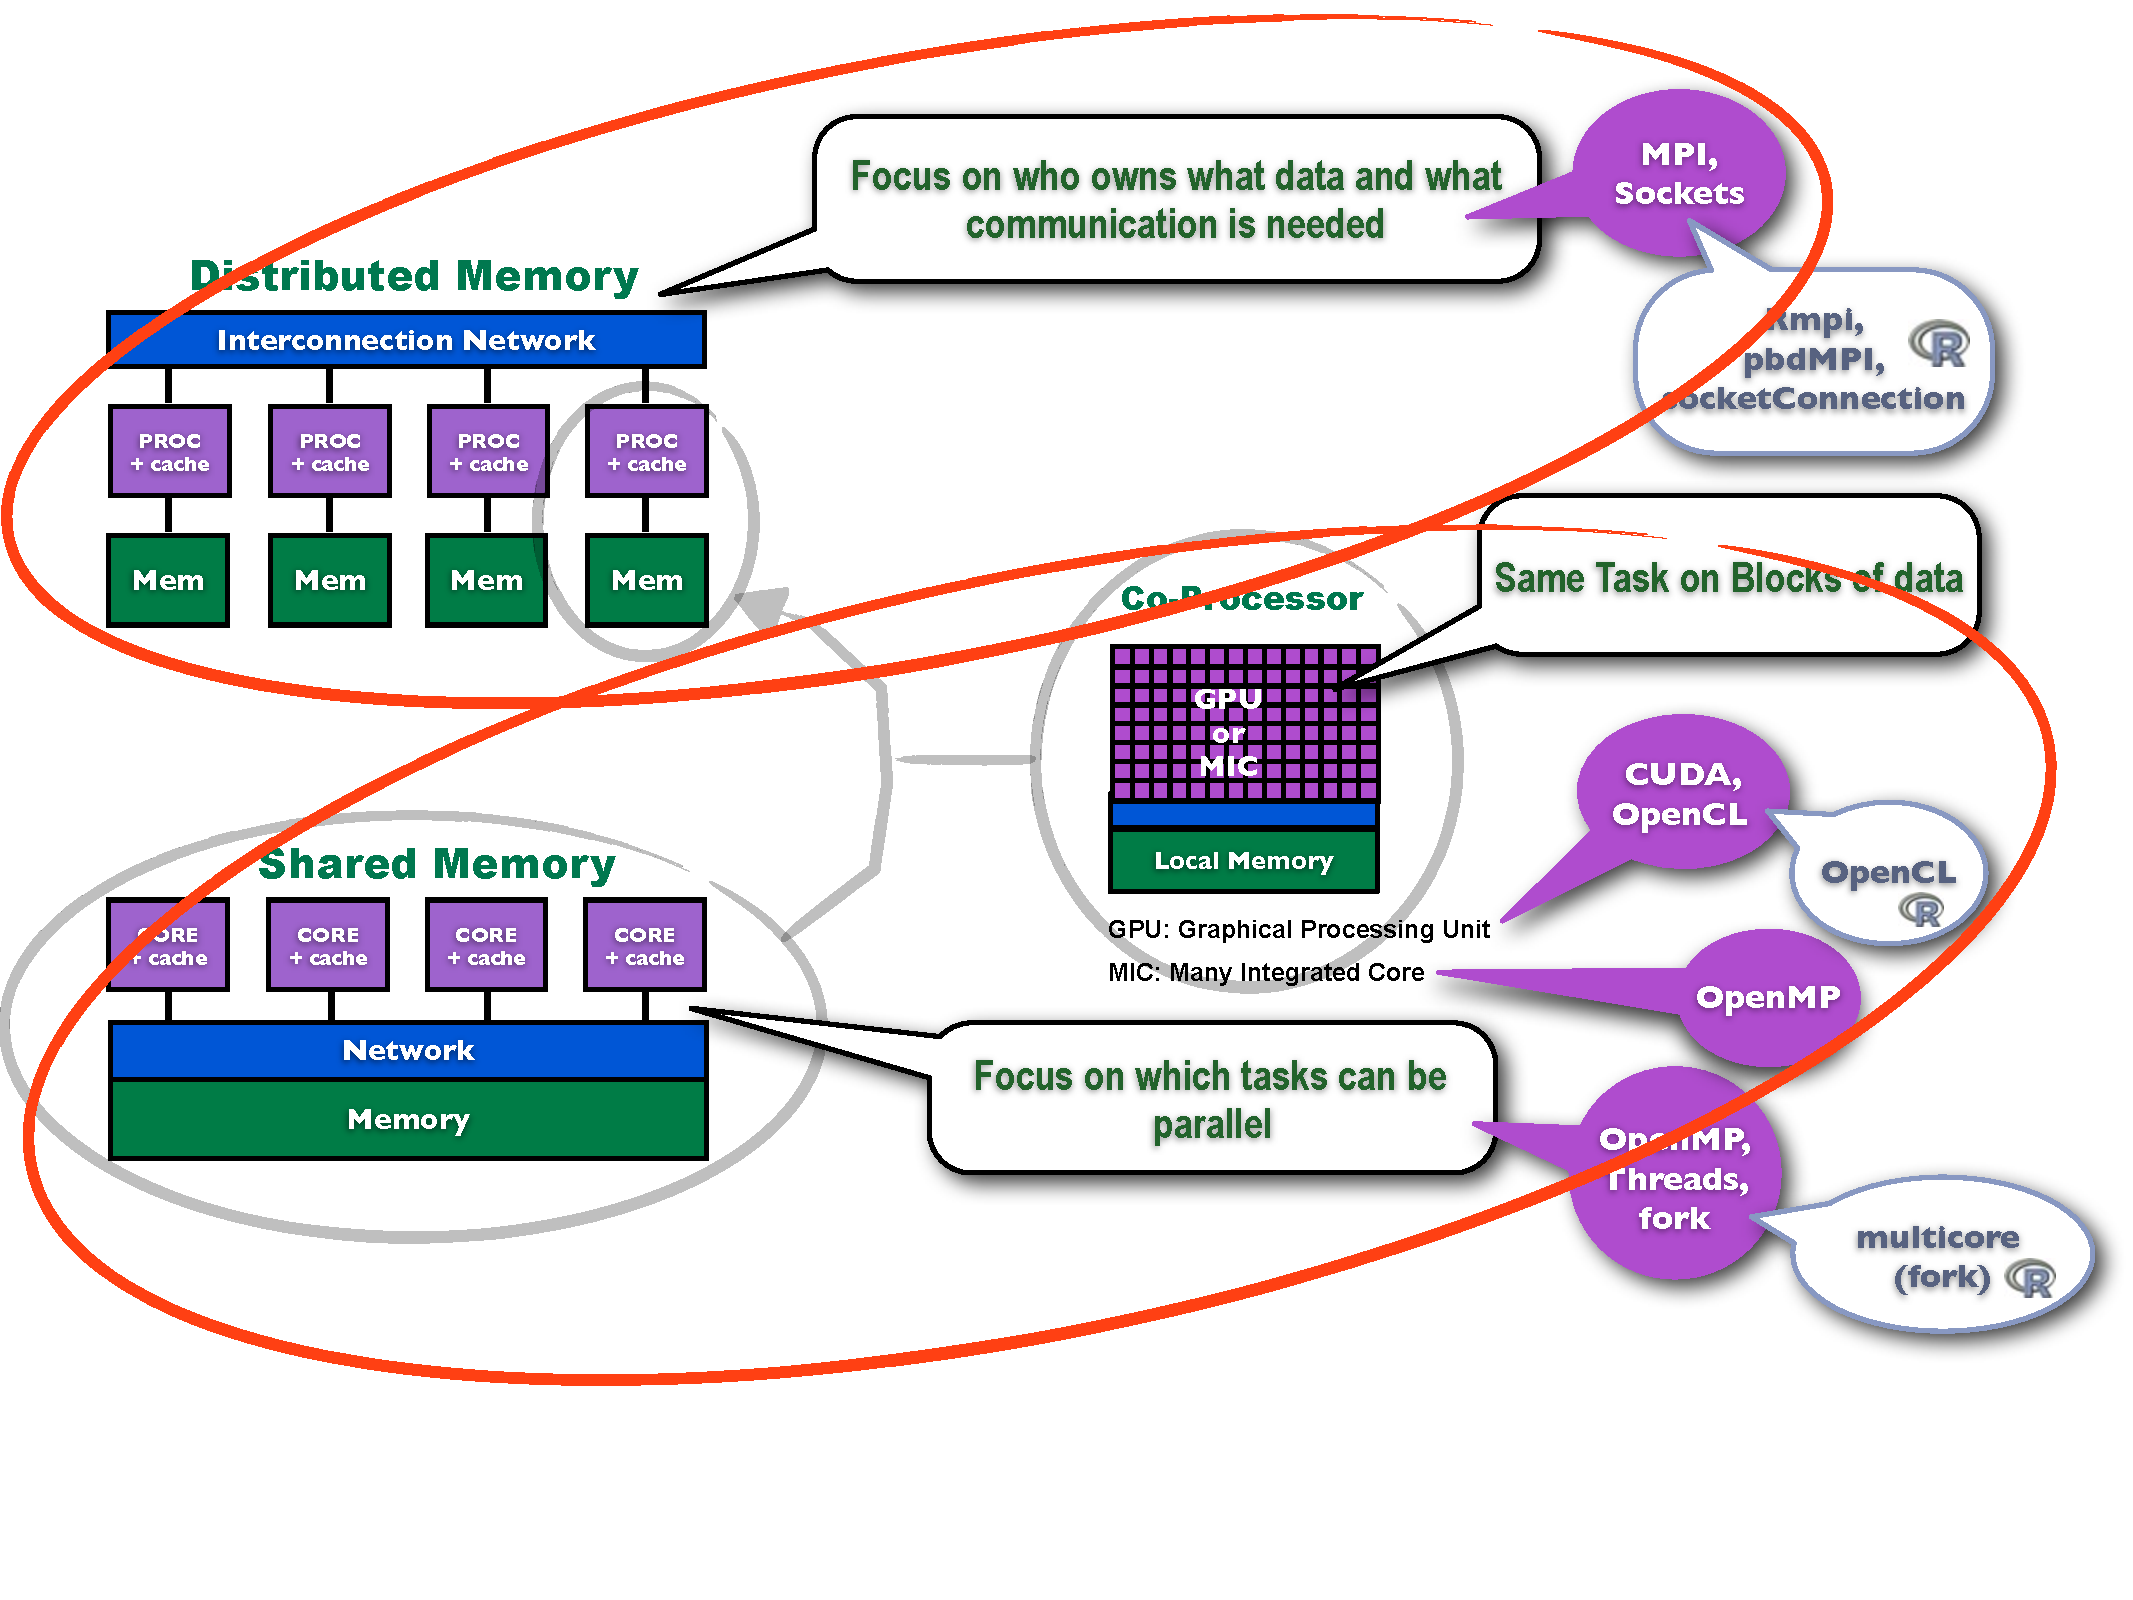
\includegraphics[width=1.30\textheight]
{../common/pics/hardware/ParallelHardware10.pdf}
\end{frame}

\begin{frame}{Big Data and Little Data}
\begin{minipage}{11cm}
  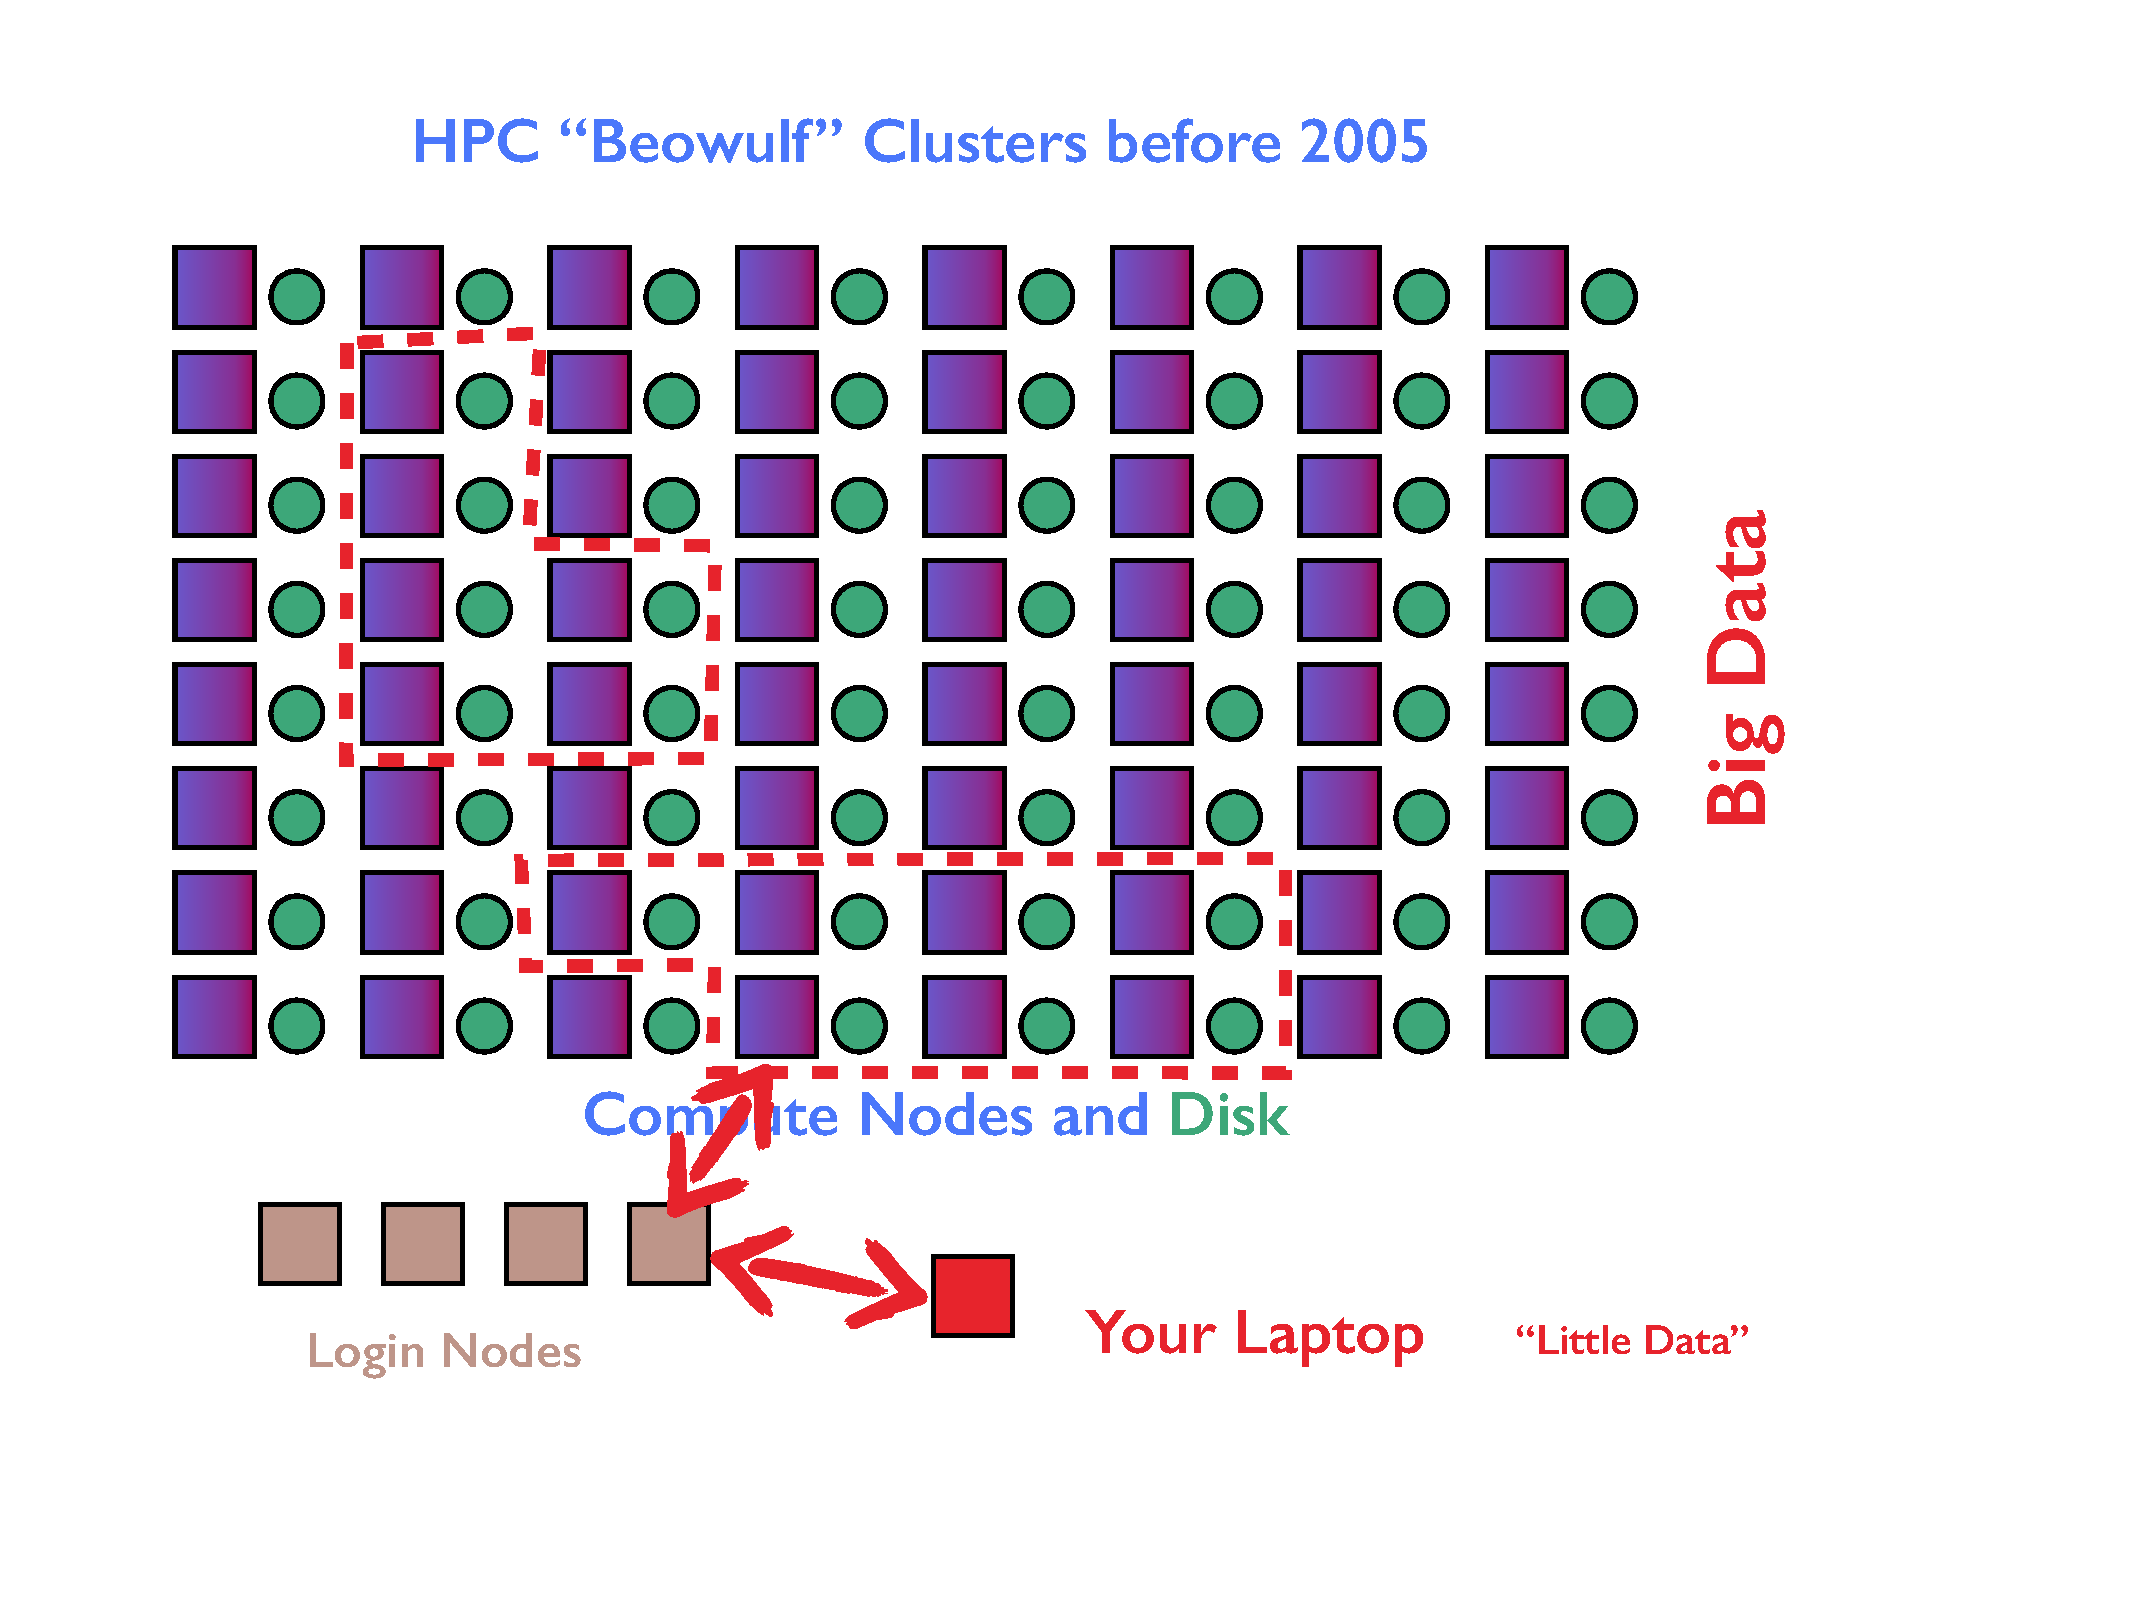
\includegraphics[width=1.25\textheight]
  {../common/pics/hardware/ParallelHardware22.pdf}\hfill
\end{minipage}
\begin{minipage}{4cm}
  \begin{block}{Analysis Workflow}\pause
    \begin{itemize}[<+-|alert@+>]
    \item Bring-in or generate data
      \begin{itemize}
      \item Write parallel data reader or data generator
      \end{itemize}
    \item Run analysis
    \item Generate graphics to display results
    \item Profile and optimize code
    \end{itemize}
  \end{block}
\end{minipage}
\end{frame}

\begin{frame}{We can work with Hadoop's HDFS $\ldots$ soon}
  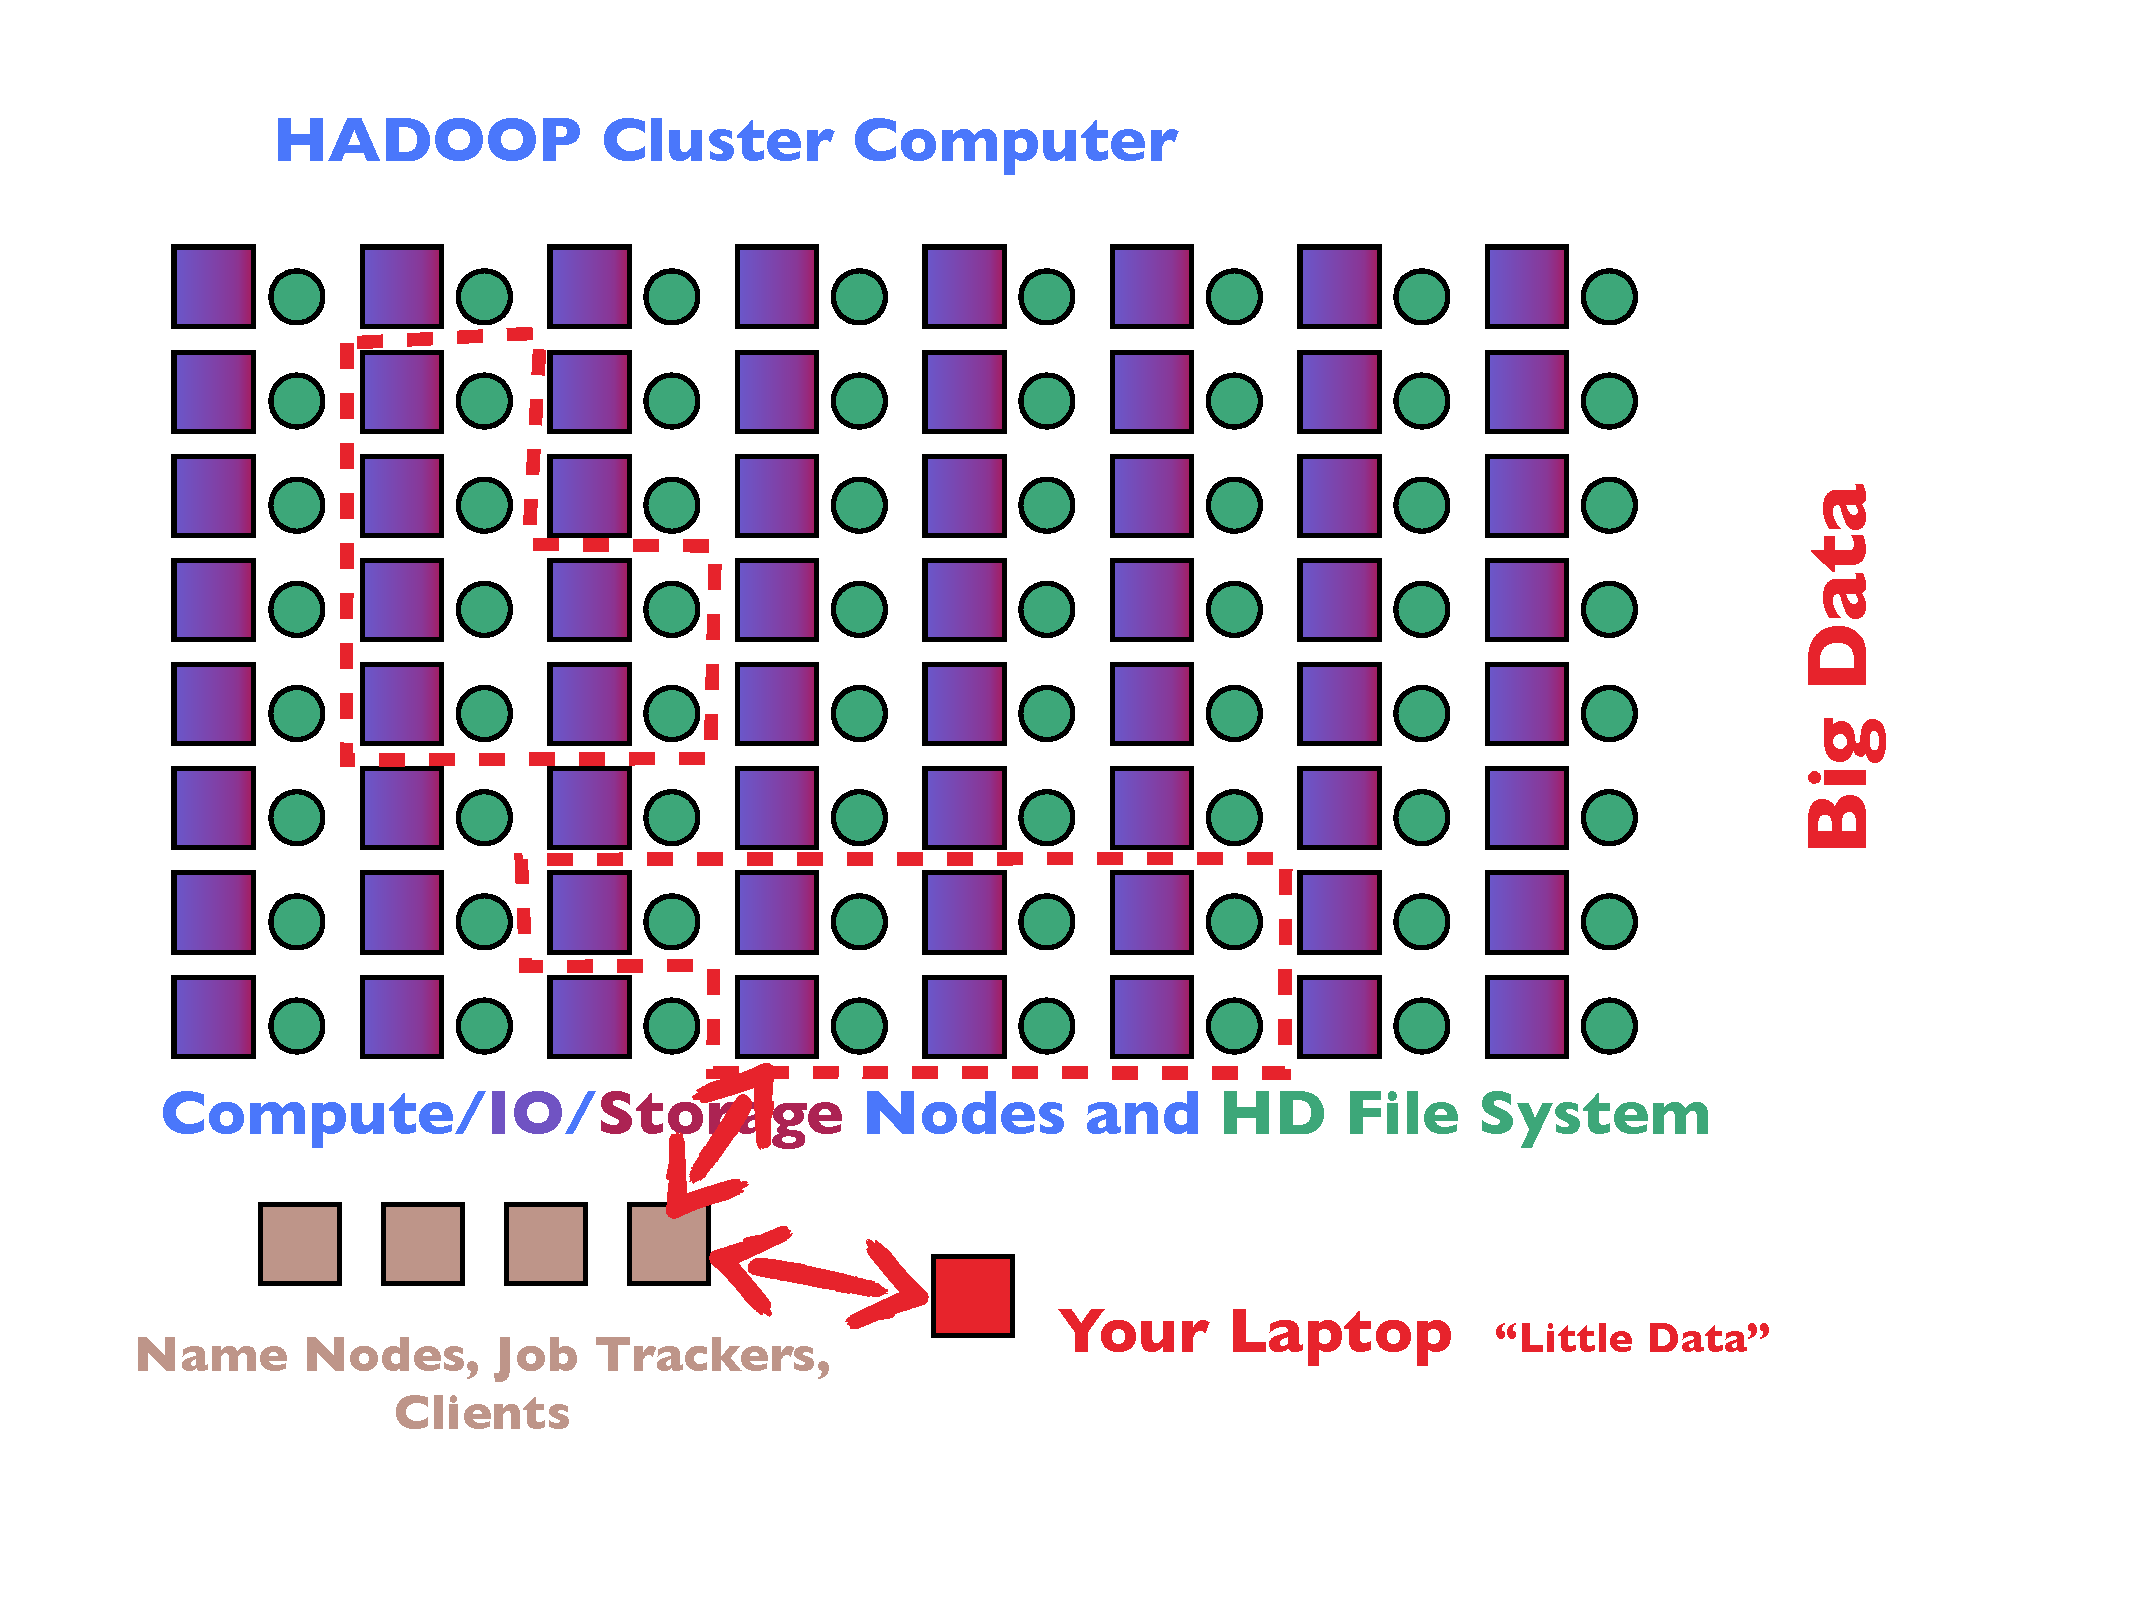
\includegraphics[width=1.25\textheight]
  {../common/pics/hardware/ParallelHardware23.pdf}
\end{frame}

\begin{frame}{R and \pbdR Interfaces to Libraries ``Standing on the Shoulders of
  Giants''}
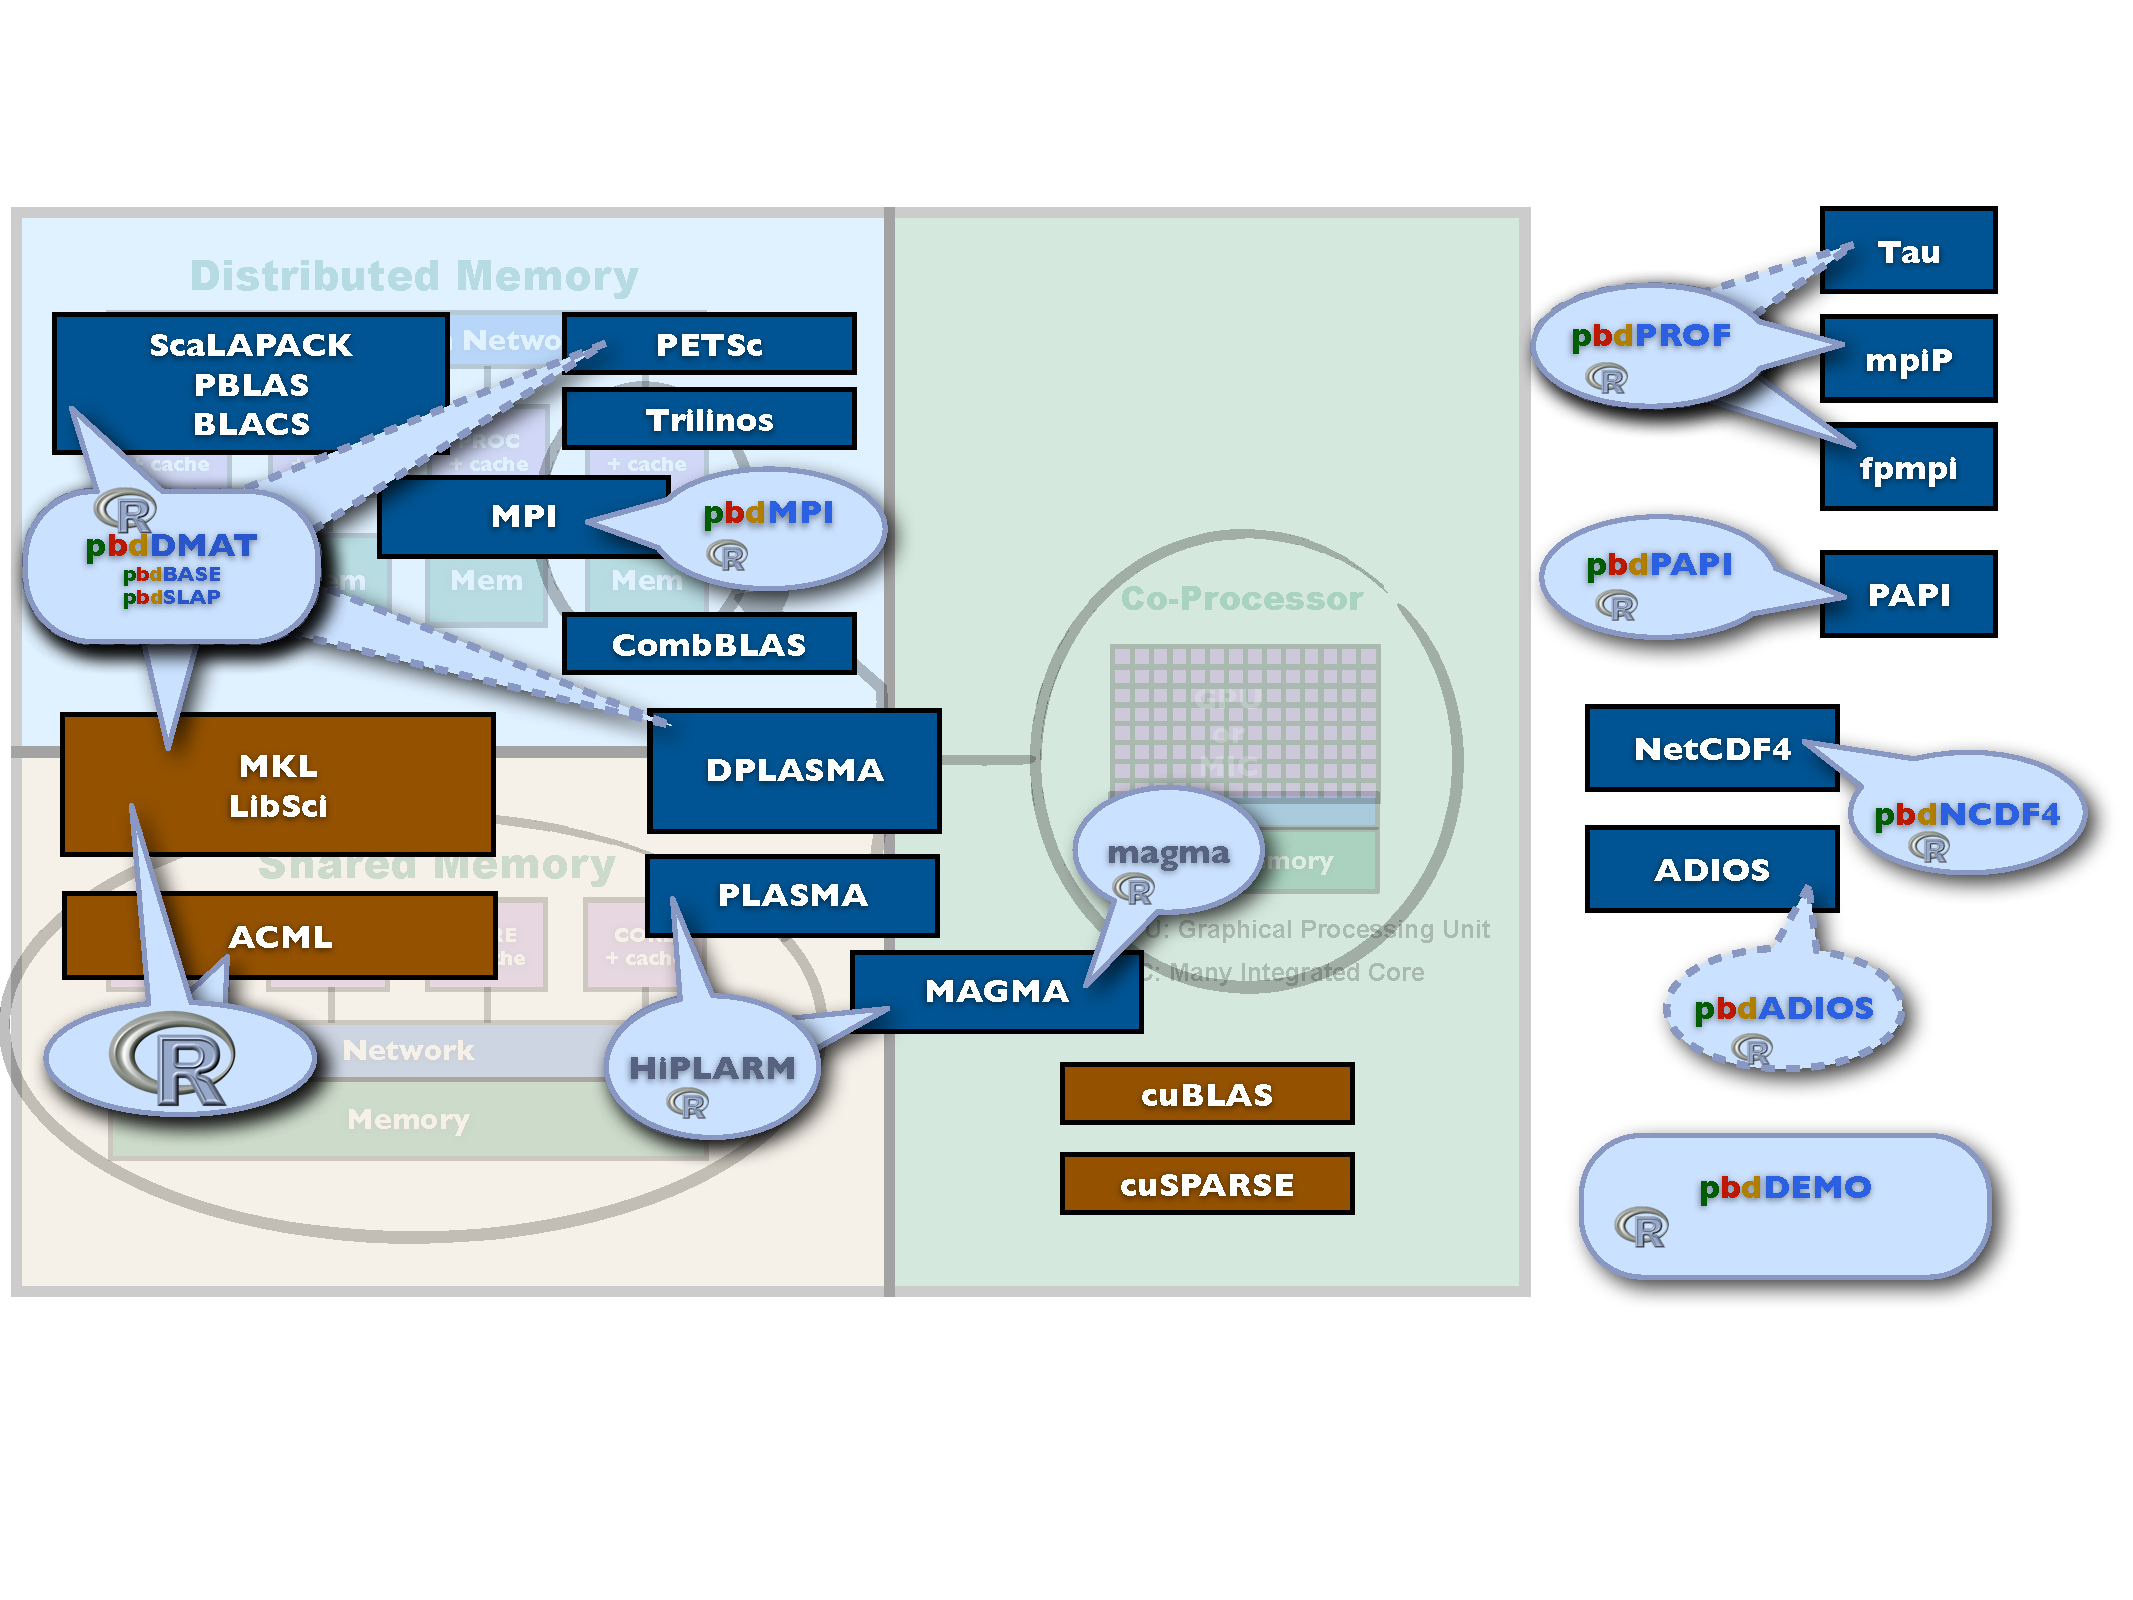
\includegraphics[width=1.35\textheight]
{../common/pics/hardware/ParallelHardware14.pdf}
\end{frame}

%\begin{frame}{Low level R Interfaces to Native Tools}
%\includegraphics[width=0.95\textheight]
%{../common/pics/hardware/ParallelHardware22.pdf}
%\includegraphics[width=0.95\textheight]
%{../common/pics/hardware/ParallelHardware23.pdf}
%\end{frame}

